\chapter{RCs without Reservoirs: Nonlinear Vector Auto-regressions}\label{ch:nvar}

In 2021, Erik Bollt proved~\cite{bollt2021} that a completely linear
ESN is mathematically equivalent to an existing tool known as a \emph{vector
auto-regression}, or VAR. He subsequently proved that an ESN with a
quadratic output nonlinearity is likewise equivalent to a
\emph{nonlinear VAR}, or NVAR.

In this chapter, I provide a brief outline of this equivalence proof,
beginning with a discussion of the behavior of fully linear ESNs as
well as their drawbacks. Later, I describe the VAR and NVAR
methods. This provides background information and motivation for the
original work presented in \cref{ch:nvar-application}.

Although output-nonlinear ESNs and NVARs are mathematically
equivalent, the conditions of their equivalence raise some practical
concerns when it comes to implementation. In this chapter discuss
these concerns, as well as the relative merits of the ESN and NVAR
approaches. In addition, I discuss how the NVAR approach benefits from
reinterpretation within the RC framework.

In \cref{ch:nvar-application} I build on the information provided
here to demonstrate the NVAR approach in practical applications, and
address these concerns about the applicability of Bollt's proof.

\section{Solutions to Linear ESNs}

\subsection{Prediction}

A fully linear ESN, with both the activation function $f$ and the
read-out function $\bm{g}$ set to the identity function, has very
simple solutions. 
As an example, I will take the discrete-time linear
ESN equation in prediction mode from \cref{tab:esn}~(d),
\begin{align}
  \bm{r}(t + \Delta t) &= (1 - \gamma \Delta t) \bm{r}(t) + \gamma \Delta t \left( W_r\;\bm{r}(t) + W_\text{in}\;W_\text{out}\;\bm{r}(t)\right), \label{eq:nvar-esn-forecast} \\
  \bm{y}(t+\Delta t) &= W_\text{out}\;\bm{r}(t+\Delta t).
\end{align}
The linear coefficients of $\bm{r}(t)$ can be collected into a single matrix
\begin{equation}
  W \equiv (1 - \gamma \Delta t) I + \gamma \Delta t \left( W_r + W_\text{in}\;W_\text{out}\right),
\end{equation}
simplifying the \cref{eq:nvar-esn-forecast} to
\begin{equation}
  \bm{r}(t + \Delta t) = W\;\bm{r}(t).
  \label{eq:nvar-esn-forecast-simple}
\end{equation}
Almost all square matrices of complex numbers are diagonalizable. If
$W$ is an $N \times N$ matrix, diagonalizing $W$ yields $N$
uncoupled time evolution equations $r_i(t + \Delta t) = w_i\;
r_i(t)$ where $w_i$ may be complex. Solutions to this equation are very simple,
\begin{equation}
  r_i(k \Delta t) = w_i^k\; r_i(0).
\end{equation}

This means the dynamics of the ESN amount to discrete-time complex
waves, possibly with an exponential growth or decay over time. This is
all the RC output layer has to draw from to construct the output
$\bm{y}(t)$. For the forecasting task, a sum of sine waves of
different frequencies can perform adequately well for short-term
prediction~\cite{bollt2021}, as this effectively amounts to a discrete
Fourier approximation. However, for long term attractor reconstruction
and the reproduction of global properties of the input system, this
linear ESN \emph{must} eventually fail on anything but the simplest
input system. The most direct demonstration of this failure is that
this linear ESN cannot predict any fixed point of the input system
except $\bm{y}(t) = 0$. It is possible to shift this fixed point to
another location by adding a constant term to
\cref{eq:nvar-esn-forecast-simple}, but this change can only move the
fixed point around, not add new ones.

To have any hope of reconstructing the underlying system attractor, as
demonstrated with ESNs in \cref{ch:low-connectivity}, an ESN must have some nonlinear component, either in the
activation function $f$ or the read-out function
$\bm{g}$. Still, a completely linear ESN is mathematically easy to
work with, and indeed the RC/NVAR equivalence proof begins by looking
at the behavior of a discrete-time linear ESN in inference mode.

\subsection{Inference}

For ESNs in inference mode, from \cref{tab:esn}~(c),
\begin{align}
  \bm{r}(t + \Delta t) &= (1 - \gamma \Delta t) \bm{r}(t) + \gamma \Delta t \left( W_r\;\bm{r}(t) + W_\text{in}\;\bm{u}(t) \right), \label{eq:nvar-esn} \\
  \bm{y}(t+\Delta t) &= W_\text{out}\;\bm{r}(t+\Delta t). \label{eq:nvar-esn-output}
\end{align}
The coefficients of $\bm{r}(t)$ and $\bm{u}(t)$ can be collected into two matrices,
\begin{align}
  A &\equiv (1 - \gamma \Delta t) I + \gamma \Delta t W_r, \\
  B &\equiv \gamma \Delta t W_\text{in}.
\end{align}
\Cref{eq:nvar-esn} then simplifies to
\begin{equation}
  \bm{r}(t + \Delta t) = B\;\bm{u}(t) + A\;\bm{r}(t).
\end{equation}
This equation is recursive; expanding it out into the past yields
\begin{align}
  \bm{r}(t + \Delta t) &= B\;\bm{u}(t) + AB\;\bm{u}(t - \Delta t) + A^2\;\bm{r}(t), \\
  \bm{r}(t + \Delta t) &= \sum_{j = 0}^\infty A^j B \bm{u}(t - j \Delta t). \label{eq:esn-var-mat}
\end{align}

\Cref{eq:esn-var-mat} states that the value of $\bm{r}(t + \Delta t)$
is constructed from a linear combination of time-delay taps of the
input $\bm{u}(t)$, extending infinitely into the past.  In combination
with \cref{eq:nvar-esn-output}, this means the overall output
$\bm{y}(t)$ is a linear combination of time-delay taps of the input
$\bm{u}(t)$.  This is known as a vector auto-regression.

\section{Linear Vector Auto-regressions (VARs)}

In most cases, the term \emph{vector auto-regression} specifically
means a method of producing an output $\bm{y}(t)$ from a linear
combination of past outputs. However, I generalize this slightly
to better mirror the reservoir computer model introduced in
\cref{ch:reservoir-computing}.

In this dissertation, a vector auto-regression (VAR) is a method of
transforming a discrete-time input signal $\bm{u}(t)$ into a
discrete-time output signal $\bm{y}(t)$ from a linear combination of
time-delay taps. Given a list of tap delays $\tau_i$, I construct
a tap vector $\bm{v}(t)$ via
\begin{equation}
  \label{eq:var-v}
  \bm{v}(t + \Delta t) = \bm{u}(t - \tau_0 \Delta t) \oplus \bm{u}(t - \tau_1 \Delta t) \oplus \cdots \oplus \bm{u}(t - \tau_{q-1} \Delta t)
\end{equation}
where the operator $\oplus$ is understood to mean vector
concatenation. That is, if the input $\bm{u}(t)$ has dimension $d$,
and if there are $q$ taps, then the vector $\bm{v}(t)$ has dimension
$dq$. Most commonly, $\tau_0 = 0$, which ensures that the VAR has access to the most recent information from $\bm{u}(t)$ when producing an output.

\begin{figure}
  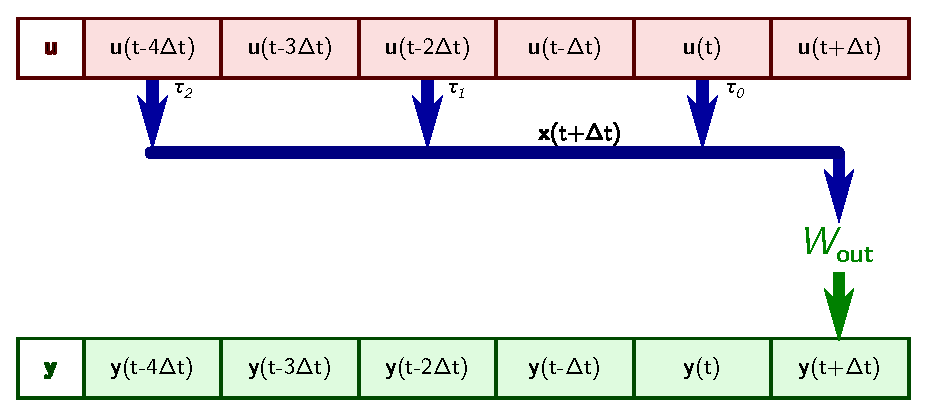
\includegraphics{figures/var-infer}
    \caption{Summary of the (N)VAR method. Many time-delay taps $\tau_i$
    of the discrete-time signal $\bm{u}(t)$ (top, red) are concatenated into the tap
    vector $\bm{v}(t)$ (middle, blue). Here, there are three taps
    $\tau_0=0$, $\tau_1=2$, and $\tau_2=4$. These taps are then passed
    through a possibly nonlinear function $\bm{g}_\text{n}$ and
    combined linearly by the output matrix $W_\text{out}$ to produce
    the next value of the (N)VAR's output $\bm{y}(t)$ (bottom,
    green). For a linear VAR, $\bm{g}_\text{n}$ is the identity
    function. To transform a whole time series input, this (N)VAR process
    slides along the time axis from left to right.}
  \label{fig:var-infer}
\end{figure}

The output of the VAR is a linear transformation of this tap vector,
\begin{equation}
  \label{eq:var-y}
  \bm{y}(t + \Delta t) = W_\text{out}\;\bm{g}_\text{n}\left(\bm{v}(t + \Delta t)\right),
\end{equation}
where $\bm{g}_\text{n}$ is the identity function. If $\bm{g}_\text{n}$
is instead chosen to be nonlinear, this results in a nonlinear VAR,
which I discuss in \cref{sec:nvar}.

This transformation process, from input to output, is summarized in
\cref{fig:var-infer}. Note the similarity to the RC method: the input
signal $\bm{u}(t)$ drives an internal state $\bm{v}(t)$ / $\bm{r}(t)$,
which is then linearly transformed into the output
$\bm{y}(t)$. However, the internal state $\bm{v}(t)$ of the VAR is
much simpler than that of most reservoirs, because it is constructed
directly from the input.

\subsection{Training and Testing}

Once the taps $\tau_i$ are selected, the VAR can be trained in much
the same way as an RC. The VAR is fed an example input
$\bm{u}_\text{train}(t)$, which produces an example tap vector
$\bm{v}_\text{train}(t)$ via \cref{eq:var-v}. Finally, a $W_\text{out}$
that best maps this $\bm{v}_\text{train}(t)$ onto the example output
$\bm{y}_\text{train}(t)$ can be found via ridge regression, exactly as
in the RC case.

VARs can also be used for forecasting as well. Analogously to the RC
case, the VAR used for forecasting can be trained to reproduce the
example input as its output. Since the VAR output $\bm{y}(t + \Delta
t)$ depends only on $\bm{u}(t)$ at time $t$ and earlier, this amounts
to one step ahead prediction. Once trained, the VAR can do autonomous
prediction by replacing the input $\bm{u}(t)$ with the output
$\bm{y}(t)$ in \cref{eq:var-v}.

For practical reasons, in this dissertation, forecasting VARs have a modified
output equation
\begin{equation}
  \bm{y}(t + \Delta t) = \bm{u}(t) + W_\text{out}\;\bm{g}_\text{n}\left(\bm{v}(t + \Delta t)\right).
\end{equation}
This effectively changes the VAR from one step ahead prediction to
predicting the difference between the last value of the signal and the
next, in analogy to a discrete-time integrator. Without this change,
the components of $W_\text{out}$ corresponding to $\bm{u}(t)$ are
larger than the others. Because the ridge regression used to find
$W_\text{out}$ has a single regularization parameter $\alpha$, it
works best when all components of $W_\text{out}$ have about the same
expected scale.

Once trained, either as a signal transformation or for prediction, a
VAR can be tested in the same ways as an RC. For signal
transformations, the VAR output is compared to the true signal,
yielding a NRMSE $\epsilon$. For prediction, the VAR can be used to
generate multiple predictions for a single Lyapunov time, and the
NRMSE $\epsilon_1$ from these predictions is combined into an average
error $\tilde{\epsilon}$.

\subsection{Comparing VARs to ESNs}

Working with a VAR, by training it and using it, is very similar to
working with an RC. The most important difference is that using a VAR
completely sidesteps the issue of choosing an internal
reservoir. Building an ESN reservoir is a complicated process that
starts with the meta-parameters listed in
\cref{tab:esn-metaparameters} and ends with a random realization of a
network, usually of 100 nodes or more. In contrast, building a VAR
amounts to selecting which taps $\tau_i$ to use, and how many. This
dramatic reduction in the parameter space makes VARs easier to build
and use, and the lack of a random component makes it possible to
deterministically specify a VAR's construction.

By describing the VAR method within the reservoir computing framework,
there are a few benefits to the VAR method as well. Previous work with
VARs has trained the $W_\text{out}$ matrix with least squares, while
work in the RC field has long used ridge regression as a way to reduce
overfitting and encourage generalization. In addition, VARs benefit
from the more sophisticated forecasting evaluation methods, such as
$\tilde{\epsilon}$, developed for use with RCs.

However, the linear ESN solution in \cref{eq:esn-var-mat} is only
completely equivalent to a VAR with an infinite number of time delay
taps. VARs with a finite number of taps $q$ approximate a VAR
with infinite taps under the right conditions as $q \rightarrow
\infty$~\cite{bollt2021}, but if VARs are to be used as a replacement
for RCs, it is critical to know how good this approximation is in
practice. If a VAR requires thousands of taps to work, it may still
be simpler just to use an ESN.

Finally, these linear VARs suffer from the same drawbacks as the
linear ESN. Any practical replacement for a full, nonlinear ESN would have to
reproduce the attractors of the systems they are trained on, as in
\cref{ch:low-connectivity}, and to do that, they need a nonlinearity.

\section{Nonlinear Vector Autoregressions (NVARs)}\label{sec:nvar}

The ESN model has two possible sources of nonlinearity: the
activation function $f$ and the read-out function $\bm{g}$. Most
commonly, including in \cref{ch:low-connectivity}, $f =
\tanh$. However, a nonlinear $f$ is mathematically difficult to work
with, as it lies in the middle of the ESN's internal state equation. In
contrast, the read-out function $\bm{g}$ sits only on the output
layer. Consider the linear ESN described in
\cref{eq:esn-var-mat} modified to have a nonlinear read-out function
\begin{equation}
  g_i(\bm{r}) = \begin{cases}
    r_i & \text{if } i \leq N, \\
    r_{i - N}^2 & \text{if } N < i \leq 2N.
  \end{cases}
  \label{eq:esn-quadratic-out}
\end{equation}
where $N$ is the number of nodes in the ESN.  That is,
$\bm{g}(\bm{r})$ contains all of the node values, as well as the
square of all the node values. This is similar to the read-out
function used in \cref{ch:low-connectivity}, except that it makes no
attempt to keep the dimension of $\bm{g}(\bm{r})$ the same as the dimension of $\bm{r}$. By
\cref{eq:esn-var-mat}, each node value is a linear combination of
time-delay taps of $\bm{u}(t)$, and so the square of a node value
contains only quadratic terms of the form $u_i(t-j\Delta
t)u_k(t-l\Delta t)$.

Putting this together, the ESN's output $\bm{y}(t)$ can written in
terms of the time-delay tap vector $\bm{v}(t)$ in \cref{eq:var-v},
using an infinite number of taps $\tau_i = i$,
\begin{equation}
  \bm{y}(t + \Delta t) = W_\text{out}\;\bm{g}_\text{n}\left(\bm{v}(t + \Delta t)\right).
\end{equation}
The nonlinear function $\bm{g}_\text{n}(\bm{v})$ has all
components of $\bm{v}$ as well as all quadratic pairs of those components,
\begin{equation}
  \label{eq:quadratic-nvar}
  \bm{g}_\text{n}(\bm{v}) = \bm{v} \oplus \ceil{\bm{v} \otimes \bm{v}}.
\end{equation}
Here, the operator $\otimes$ denotes the outer product, and $\ceil{X}$
denotes the a flattened vector that contains the upper-triangular
components of $X$. For example, $\ceil{\bm{v} \otimes \bm{v}}$ is a
vector that contains as components all unique terms of the form $v_i
v_j$.

This construction, a VAR that wraps the delay tap vector in a
nonlinear function $\bm{g}_\text{n}$ before the building the linear
combination for the output, is known as a nonlinear VAR (NVAR). This
concludes a sketch of Bollt's proof that a linear ESN with quadratic
read-out is mathematically equivalent to an NVAR with infinite
taps~\cite{bollt2021}. Because the read-out function appears only on
the output, it is not difficult to change the nature of the nonlinear
read-out $\bm{g}$ in an ESN and derive the corresponding NVAR $\bm{g}_\text{n}$,
and therefore this proof generalizes easily to read-out functions that are more
complicated than quadratic.

It is important to note at this point that the ESN's output weights
$W_\text{out}$ and read-out $\bm{g}$ are \emph{not} the same as the
equivalent NVAR's output weights $W_\text{out}$ and nonlinearity
$\bm{g}_\text{out}$. In this example, the ESN's $\bm{g}$ produces node values and squares of node
values, while the NVAR's $\bm{g}_\text{n}$ produces all linear and
quadratic terms it is possible to construct from the tap vector
$\bm{v}$. The NVAR has quadratic terms that mix both the dimensions of the input $\bm{u}(t)$ as well as mix the tap delays $\tau_i$. In a practical application with a finite tap vector, this
means that if $\bm{v}$ has $q$ taps and $\bm{u}$ is dimension $d$, then $\bm{g}_\text{n}$ will have
$qd + qd(qd+1)/2$ components. This quadratic dependence on $qd$ can
rapidly cause the computational cost of the ridge regression to find $W_\text{out}$ to be very
expensive, as either the number of taps or the input dimension increases.

Putting all the pieces together, the NVAR method for transforming an
input $\bm{u}(t)$ into an output $\bm{y}(t)$ is described by
\begin{align}
  \label{eq:nvar}
  \bm{v}(t + \Delta t) &= \bm{u}(t - \tau_0 \Delta t) \oplus \bm{u}(t - \tau_1 \Delta t) \oplus \cdots \oplus \bm{u}(t - \tau_{k-1} \Delta t), \\
  \label{eq:nvar-out}
  \bm{y}(t + \Delta t) &= W_\text{out}\;\bm{g}_\text{n}\left(\bm{v}(t + \Delta t)\right).
\end{align}
For forecasting tasks, the output \cref{eq:nvar-out} is replaced with
\begin{equation}
  \label{eq:nvar-out-forecast}
  \bm{y}(t + \Delta t) = \bm{u}(t) + W_\text{out}\;\bm{g}_\text{n}\left(\bm{v}(t + \Delta t)\right).
\end{equation}

Simply by wrapping the tap vector $\bm{v}$ in a nonlinear function
before the output, the NVAR now has the nonlinearity required to have
any hope of reproducing attractors as well as the nonlinear ESNs, and
in \cref{ch:nvar-application} I demonstrate that NVARs perform
quite well in this role.

\section{Practical Considerations}

The above sketch of Bollt's proof demonstrates that a linear ESN with nonlinear
readout is equivalent to an NVAR with an infinite number of taps. In
practice, though, this method can only be implemented with a finite
number of taps. If an NVAR implementation requires thousands of taps
to work, it is not a realistic replacement for the ESN method.

The number of taps $q$ and input dimension $d$ are also relevant for the quadratic
$\bm{g}_\text{n}$ described in \cref{eq:quadratic-nvar}. The output
dimension of this function, $qd + qd(qd + 1)/2$, is also one of the
dimensions of the output matrix $W_\text{out}$. As this dimension
grows, so does the time required to perform ridge regression. This
quadratic dependence on $q$ also emphasizes the need to keep the
number of taps low.

On top of this, a quadratic output may not be enough. If a quadratic
NVAR is trained to do forecasting on a system with total inversion
symmetry $\bm{u}(t) \rightarrow -\bm{u}(t)$, the quadratic terms in
the output cannot meaningfully contribute. This reduces the NVAR to a
linear VAR, with all the forecasting problems that entails. To use an
NVAR on such a system, the nonlinear function $\bm{g}_\text{n}$ must
be expanded to include higher-order terms. This can be done by
constructing an ESN and calculating the equivalent NVAR form, but it
can also be done more directly by simply adding higher-order monomial terms to
$\bm{g}_\text{n}$. I explore this in
\cref{ch:nvar-application}. However, this further emphasizes the
requirement for a small number of taps, as the number of terms of
order $n$ grows as $(qd)^n$.

\begin{table}
  \caption{Summary of NVAR parameters. Compared to the ESN approach in
    \cref{tab:esn-metaparameters}, the NVAR method is much simpler.}
  \begin{tabularx}{\linewidth}{rlX}
    & Parameter & Description \\
    \hline
    \rule{0pt}{4ex}
    $\tau_i$ & Tap Delays & the placement of time-delay taps \\
    \rule{0pt}{4ex}
    $\bm{g}_\text{n}$ & Read-out Function & the nonlinearity on the output layer \\
    \rule{0pt}{4ex}
    $\Delta t$ & Time Step & the discrete time step of both the input $\bm{u}(t)$ and the NVAR itself \\
    \rule{0pt}{4ex}
    $\alpha$ & Ridge Parameter & regularization parameter for ridge regression \\
  \end{tabularx}
  \label{tab:nvar-parameters}
\end{table}

If these challenges can be overcome, NVARs are an extremely appealing
replacement for the ESN approach. ESNs are complicated random networks
with many poorly-understood meta-parameters. In contrast, NVARs have
only four total parameters, listed in \cref{tab:nvar-parameters}.  In
addition to being a smaller set of parameters, these parameters are
simply much more interpretable. It is not straightforward to imagine
what changing the input connectivity of an ESN will do to performance,
but changing the taps $\tau_i$ has a direct effect on what information
is available to the NVAR.

\section{Summary}

VARs and NVARs are, like RCs, a method of transforming an input signal
into an output signal. They operate on linear combinations of
time-delay taps of the input. In many ways, their construction and use
mirrors that of an RC, except that there is no internal dynamic
reservoir system. This sidesteps a whole host of questions and
decisions relating to reservoir construction, and dramatically
simplifies the implementation of VARs and NVARs. However, despite this
simplicity, they are now known to be mathematically equivalent to an
output layer nonlinear ESN.

% FIXME cite nvar
NVARs are an existing method, but they are not widely used or discussed. This equivalence opens the door
to cross-talk between the NVAR and RC communities. On the RC side,
researchers gain a dramatically simpler implementation that is known
to be equivalent, and also gain a chance to apply lessons learned in
the RC world to the NVAR method. The NVAR approach benefits from the
use of ridge regression, long used in the RC field, instead of other
linear fitting methods.  It also benefits from improvements to
evaluation, such as $\tilde{\epsilon}$, and opens the door to using
NVARs on traditional RC problems. However, some questions still
remain -- most notably, how many time-delay taps are practically
necessary, and how complicated a nonlinear function will most tasks
need?

If these questions are resolved, the NVAR approach is an extremely
attractive alternative to the ESN approach. NVARs do not rely on
random construction, are simple to implement, and have only a few
parameters with direct interpretations. If NVARs work well, it becomes
difficult to recommend ESNs and the complications they entail.

In the next chapter, I apply the NVAR method to the traditional
RC tasks of system state inference and chaotic system forecasting. In
the process, I resolve these remaining questions, and demonstrate
that NVARs are a practical and very simple replacement for traditional
ESN approaches.
